\section{Idiotenseite}
\subsection{Log-Tabelle}\label{log_tabelle}
\begin{center}
	\parbox{7cm}{
		\scriptsize
	\begin{tabular}{l|l|l|l}
		\textbf{Lrel. (dB)} & \textbf{Lrel. (NP)} & \textbf{P2/P1} & \textbf{A2/A1} \\ \toprule
		$100.000$ & $11.513$ & $10^{10}$ & $10^5$ \\ \hline
		$90.000$ & $10.362$ & $10^9$ & $31622.777$ \\ \hline
		$80.000$ & $9.210$ & $10^8$ & $10^4$ \\ \hline
		$70.000$ & $8.059$ & $10^7$ & $3162.278$ \\ \hline
		$60.000$ & $6.908$ & $10^6$ & $10^3$ \\ \hline
		$50.000$ & $5.756$ & $10^5$ & $316.228$ \\ \hline
		$40.000$ & $4.605$ & $10^4$ & $10^2$ \\ \hline
		$30.000$ & $3.454$ & $10^3$ & $31.623$ \\ \hline
		\textbf{$20.000$} & $2.303$ & \textbf{$10^2$} & \textbf{$10.000$} \\ \hline
		$19.085$ & $2.197$ & $81.000$ & $9.000$ \\ \hline
		$19.000$ & $2.187$ & $79.433$ & $8.913$ \\ \hline
		$18.062$ & $2.079$ & $64.000$ & $8.000$ \\ \hline
		$18.000$ & $2.072$ & $63.096$ & $7.943$ \\ \hline
		$17.000$ & $1.957$ & $50.119$ & $7.079$ \\ \hline
		$16.902$ & $1.946$ & $49.000$ & $7.000$ \\ \hline
		$16.000$ & $1.842$ & $39.811$ & $6.310$ \\ \hline
		$15.563$ & $1.792$ & $36.000$ & $6.000$ \\ \hline
		$15.000$ & $1.727$ & $31.623$ & $5.623$ \\ \hline
		$14.000$ & $1.612$ & $25.119$ & $5.012$ \\ \hline
		\textbf{$13.979$} & $1.609$ & \textbf{$25.000$} & \textbf{$5.000$} \\ \hline
		$13.000$ & $1.497$ & $19.953$ & $4.467$ \\ \hline
		\textbf{$12.041$} & $1.386$ & \textbf{$16.000$} & \textbf{$4.000$} \\ \hline
		\textbf{$12.000$} & $1.382$ & $15.849$ & $3.981$ \\ \hline
		$11.000$ & $1.266$ & $12.589$ & $3.548$ \\ \hline
		\textbf{$10.000$} & $1.151$ & \textbf{$10.000$} & $3.162$ \\ \hline
		$9.542$ & $1.099$ & $9.000$ & $3.000$ \\ \hline
		$9.000$ & $1.036$ & $7.943$ & $2.818$ \\ \hline
		$8.000$ & $0.921$ & $6.310$ & $2.512$ \\ \hline
		$7.000$ & $0.806$ & $5.012$ & $2.239$ \\ \hline
		\textbf{$6.021$} & \textbf{$0.693$} & \textbf{$4.000$} & \textbf{$2.000$} \\ \hline
		$6.000$ & $0.691$ & $3.981$ & $1.995$ \\ \hline
		$5.000$ & $0.576$ & $3.162$ & $1.778$ \\ \hline
		$4.000$ & $0.461$ & $2.512$ & $1.585$ \\ \hline
		\textbf{$3.010$} & \textbf{$0.347$} & \textbf{$2.000$} & \textbf{$1.414$} \\ \hline
		$3.000$ & $0.345$ & $1.995$ & $1.413$ \\ \hline
		$2.000$ & $0.230$ & $1.585$ & $1.259$ \\ \hline
		$1.000$ & $0.115$ & $1.259$ & $1.122$ \\ \hline
		$0.000$ & $0.000$ & $1.000$ & $1.000$ \\ \hline
		-$1.000$ & -$0.115$ & $0.794$ & $0.891$ \\ \hline
		-$2.000$ & -$0.230$ & $0.631$ & $0.794$ \\ \hline
		-$3.000$ & -$0.345$ & $0.501$ & $0.708$ \\ \hline
		-$4.000$ & -$0.461$ & $0.398$ & $0.631$ \\ \hline
		-$5.000$ & -$0.576$ & $0.316$ & $0.562$ \\ \hline
		-$6.000$ & -$0.691$ & $0.251$ & $0.501$ \\ \hline
		-$7.000$ & -$0.806$ & $0.200$ & $0.447$ \\ \hline
		-$8.000$ & -$0.921$ & $0.158$ & $0.398$ \\ \hline
		-$9.000$ & -$1.036$ & $0.126$ & $0.355$ \\ \hline
		-$10.000$ & -$1.151$ & $0.100$ & $0.316$ \\ \hline
		-$15.000$ & -$1.727$ & $0.032$ & $0.178$ \\ \hline
		-$20.000$ & -$2.303$ & $10^{-2}$ & $0.100$ \\ \hline
		-$30.000$ & -$3.454$ & $10^{-3}$ & $0.032$ \\ \hline
		-$40.000$ & -$4.605$ & $10^{-4}$ & $0.010$ \\ \hline
		-$50.000$ & -$5.756$ & $10^{-5}$ & $0.003$ \\ \hline
		-$60.000$ & -$6.908$ & $10^{-6}$ & $0.001$ \\ \hline
		-$70.000$ & -$8.059$ & $10^{-7}$ & $0.000$ \\ \hline
		-$80.000$ & -$9.210$ & $10^{-8}$ & $10^{-4}$ \\ \hline
		-$90.000$ & -$10.362$ & $10^{-9}$ & $3.162 \cdot 10^{-5}$ \\ \hline
		-$100.000$ & -$11.513$ & $10^{-10}$ & $10^{-5}$ \\ \hline
	\end{tabular}
}
\end{center}

\subsection{LinAlg}
\subsubsection{Diagonalisieren}\label{charakteristischempolynom}
Diagonalmatrix $A = TAT^{-1}$ von Matrix $A$ besteht aus Transformationsmatrix $T$, wobei $T$ die Eigenbasis $T = \begin{pmatrix}
	\vec{v}_1 & \dots  &\vec{v}_n
\end{pmatrix}$ ist.
\[D = \begin{pmatrix}
	\lambda_1 & \dots & 0 \\
	\vdots & \ddots & \vdots \\
	0 & \dots & \lambda_n \\
\end{pmatrix}\]
~\\
\noindent\textbf{Beispiel}
$A = \begin{pmatrix} -2 & 7 \\ -1 & 6 \end{pmatrix}$
\\ \\
\noindent \textbf{Eigenwert} $\lambda_n$ mit $\det(A - \textcolor{red}{\lambda} E) = 0$:
\[\det\begin{pmatrix}
	-2 - \lambda & 7 \\
	-1 & 6 - \lambda
\end{pmatrix} \Rightarrow \lambda^2 - 4\lambda - 5 = 0\]
\[{\scriptstyle \lambda_1 = -1; \lambda_2 = 5}\]
\noindent \textbf{Eigenvektoren} $\vec{v}_n$ bestimmen durch einsetzen von $\lambda_n$ in Char.Polynom und lösen von $(A - \lambda_n E)\vec{v} = 0$. \textbf{Achtung:} $\lambda$ von klein nach gross sortieren!
\begin{align*}
	\lambda_1 := \begin{pmatrix}
		-2 +1 & 7 \\
		-1 & 6 +1
	\end{pmatrix}\vec{v} &= \vec{0} &\xRightarrow{\text{Gauss}} \begin{pmatrix}
	 v_{1} = 7v_{2} \\
	 v_2 = v_2
\end{pmatrix}  = \begin{pmatrix}
	7 \\1 
\end{pmatrix}\\
 	\lambda_2 := \begin{pmatrix}
		-2 - 5 & 7 \\
		-1 & 6 - 5
	\end{pmatrix}\vec{v} &= \vec{0} &\xRightarrow{\text{Gauss}} \begin{pmatrix}
	v_{1} = v_{2} \\
	v_2 = v_2
\end{pmatrix}= \begin{pmatrix}
1 \\1 
\end{pmatrix}
\end{align*}
Mit beliebigem $\vec{v}_n$ wird nun die Transpornierte Matrix $T$ bestummen:
\[
T = \begin{pmatrix}
	\overbrace{7}^{\vec{v}_1} & \overbrace{1}^{\vec{v}_2} \\
	1 & 1
\end{pmatrix} \qquad T^{-1}=\frac{1}{6}\begin{pmatrix}
1 & -1 \\ -1 & 7
\end{pmatrix}
\]

Damit gilt $A = TDT^{-1}$

\subsection{Inverse Matrix}\label{inversematrix}
Matrix $A$ ist genau dann invertierbar, wenn $\det(A) \neq 0$. 

\[
\begin{array}{|c|c|} \hline A & E \\ \hline \end{array} \xrightarrow{Gauss}
\begin{array}{|c|c|} \hline E & A^{-1} \\ \hline \end{array} 
\]

\noindent
Spezial-Fall (2x2):
\[
A = \begin{pmatrix}
	a & b \\
	c & d \\
\end{pmatrix}
\Rightarrow 
A^{-1} =\frac{1}{det(A)}
\begin{pmatrix}
	d & -b \\
	-c & a \\
\end{pmatrix}
\]

\noindent
Spezial-Fall (3x3):

\[A=\begin{pmatrix} 
	a & b & c \\
	d & e & f \\
	g & h & i \\
\end{pmatrix}  \Rightarrow \] \[A^{-1} = \frac{1}{det(A)}
\begin{pmatrix} 
	+\underbrace{\left|\begin{array}{rr} e & f \\ h & i \\ \end{array}\right|}_{det(A_{11})} &
	-\underbrace{\left|\begin{array}{rr} b & c \\ h & i \\ \end{array}\right|}_{det(A_{21})} &
	+\underbrace{\left|\begin{array}{rr} b & c \\ e & f \\ \end{array}\right|}_{det(A_{31})} \\
	
	-\underbrace{\left|\begin{array}{rr} d & f \\ g & i \\ \end{array}\right|}_{det(A_{12})} &
	+\underbrace{\left|\begin{array}{rr} a & c \\ g & i \\ \end{array}\right|}_{det(A_{22})} &
	-\underbrace{\left|\begin{array}{rr} a & c \\ d & f \\ \end{array}\right|}_{det(A_{32})} \\
	
	+\underbrace{\left|\begin{array}{rr} d & e \\ g & h \\ \end{array}\right|}_{det(A_{13})} &
	-\underbrace{\left|\begin{array}{rr} a & b \\ g & h \\ \end{array}\right|}_{det(A_{23})} &
	+\underbrace{\left|\begin{array}{rr} a & b \\ d & e \\ \end{array}\right|}_{det(A_{33})} \\
\end{pmatrix}\]
\clearpage
\subsection{PN und Bode von UTF}\label{pn}
\begin{center}
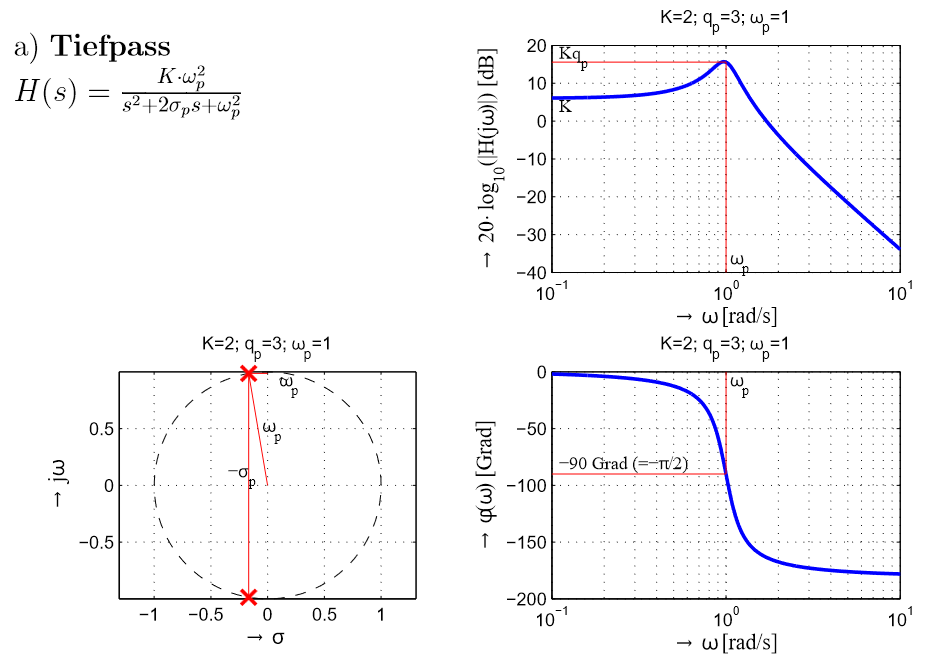
\includegraphics[width=0.8\columnwidth]{Images/tiefpass}\\
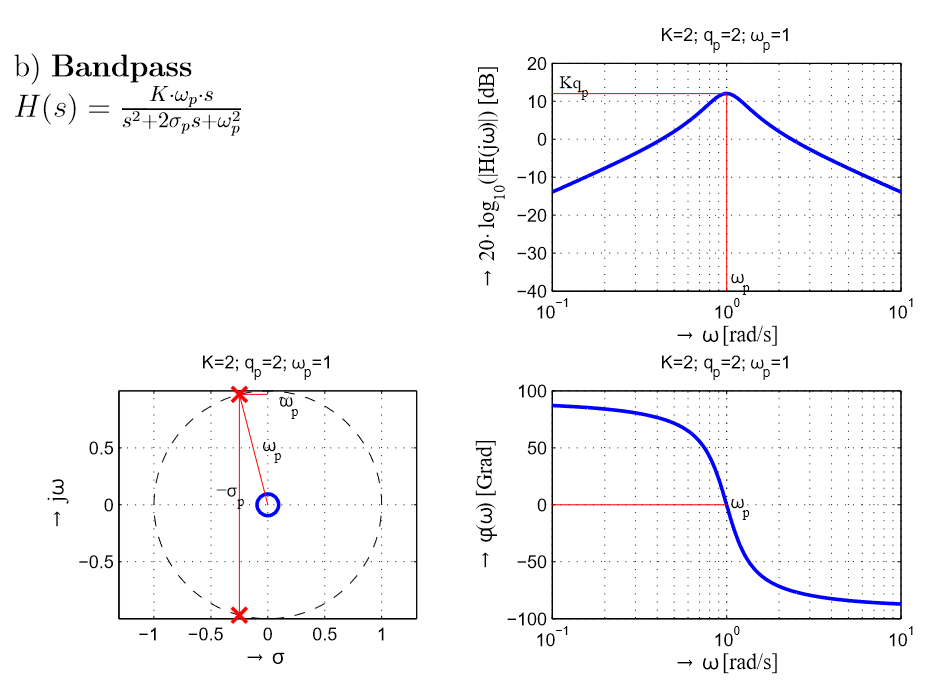
\includegraphics[width=0.8\columnwidth]{Images/bandpass}\\
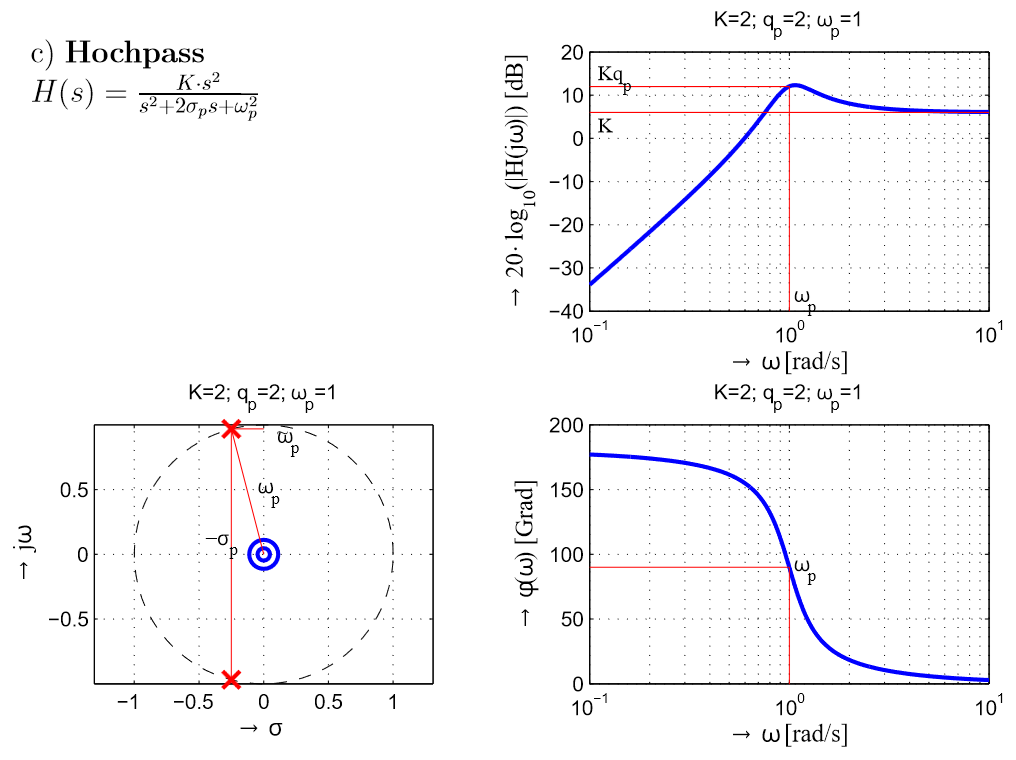
\includegraphics[width=0.8\columnwidth]{Images/hochpass}\\
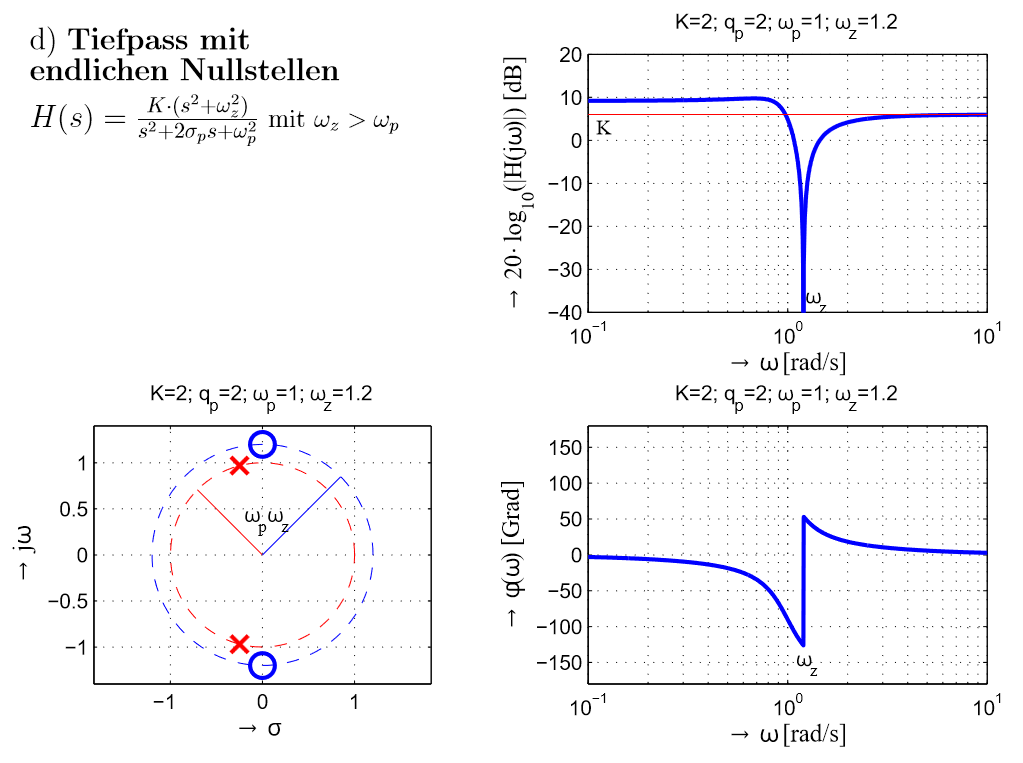
\includegraphics[width=0.8\columnwidth]{Images/tiefpass_en}\\
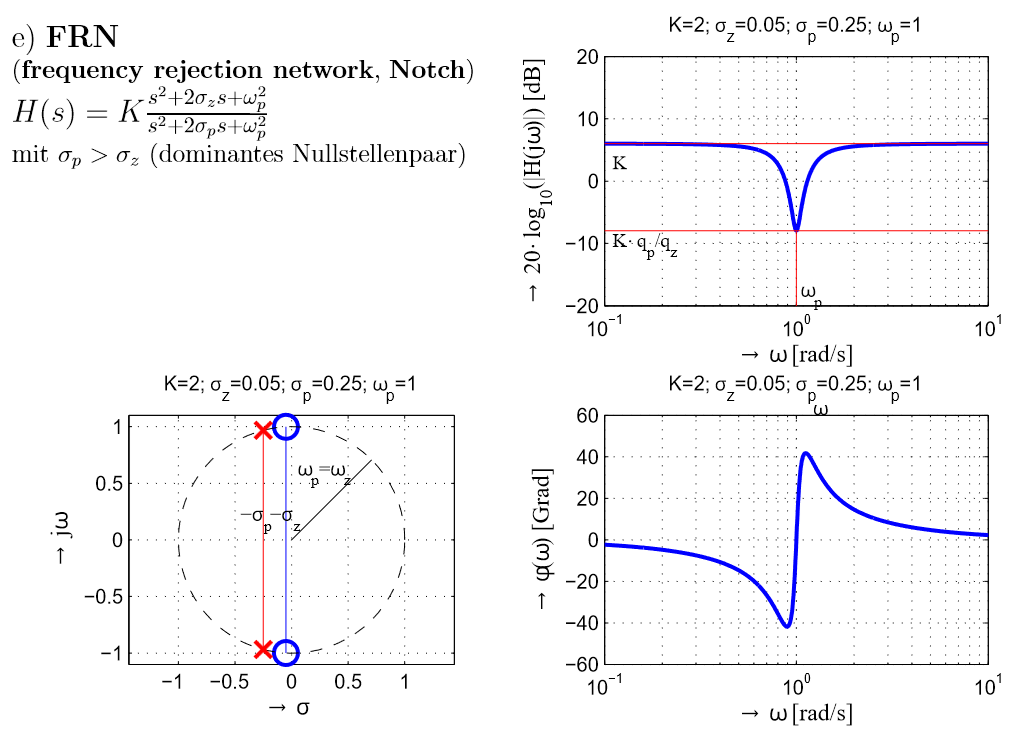
\includegraphics[width=0.8\columnwidth]{Images/frn}\\
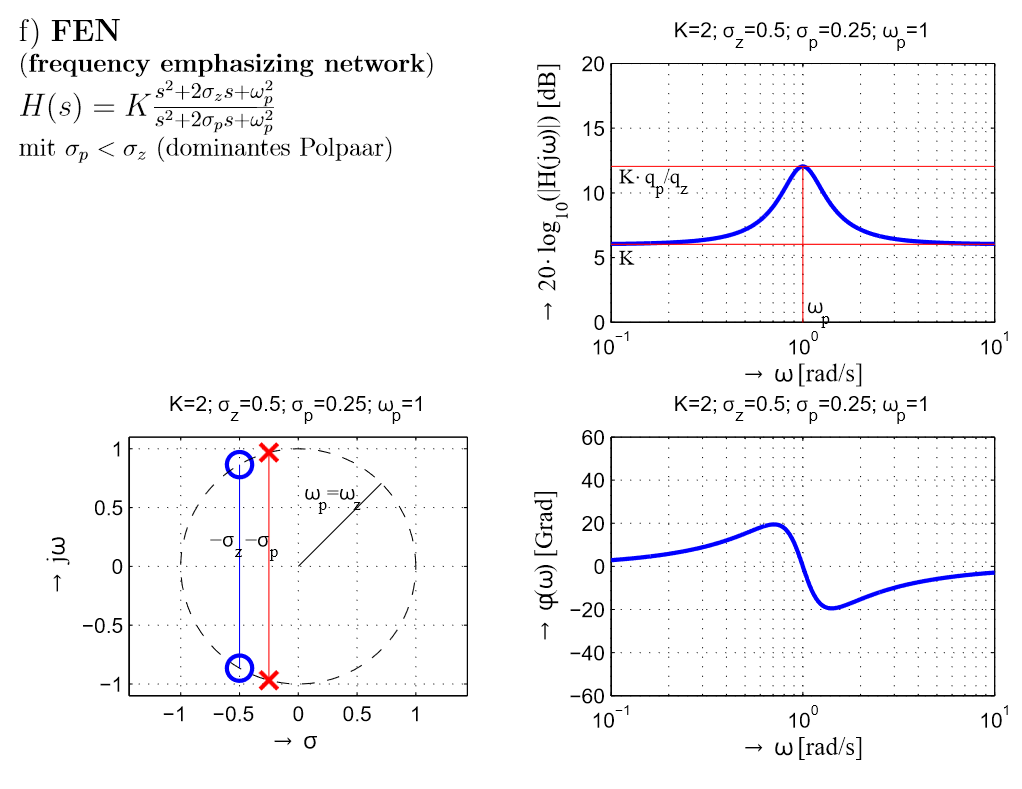
\includegraphics[width=0.8\columnwidth]{Images/fen}\\
\end{center}
